
\subsection{ESB}
\label{esb:introduccion}

\todo{Hablar de IAE}

Uno de los 9 principios de diseño de \gls{acro:soa} que mencionamos antes es el bajo acoplamiento (\eng{loose coupling}) de los servicios, y una de las formas más comunes de implementarlo es mediante un \gls{acro:esb}.

Un \gls{acro:esb} no implementa en sí mismo una arquitectura orientada a servicios, sino que proporciona las características mediante las cuales puede implementarse. Proporciona una capa de abstracción para los \eng{endpoints}, de esta manera se consigue flexibilidad y una fácil conexión entre los servicios. Existen diferentes opiniones acerca del rol exacto y de las responsabilidades de un \gls{acro:esb}, principalmente porque hay diferentes aproximaciones técnicas para realizar un \gls{acro:esb}\cite[p.~47]{josuttis2007}.

En función de los enfoques técnicos y de organización adoptados para la aplicación del \gls{acro:esb}, este puede implicar una o más de las siguientes tareas:

\begin{itemize}
  \item Proveer conectividad.
  \item Transformar la información.
  \item Ruteo (\eng{Routing}) inteligente.
  \item Manejo de aspectos de seguridad.
  \item Lidiar con la fiabilidad de los servicios.
  \item Manejo de los servicios.
  \item Monitoreo y registro de actividades (\eng{logging}).
\end{itemize}

El rol principal de estas herramientas es proveer interoperabilidad. Debido a que integran diferentes plataformas y lenguajes de programación, una parte fundamental de esta función es la transformación de datos.
Otra tarea fundamental de un \gls{acro:esb} es el ruteo, ya que debe existir alguna manera de acceder desde un consumidor a un proveedor de servicios y luego se debe poder enviar la respuesta de regreso desde el proveedor hacia el consumidor. Dependiendo de la tecnología utilizada y el nivel de inteligencia proporcionado, esta tarea puede ser trivial o puede tornarse compleja.

Hay que tener en cuenta que no existe requerimiento alguno para que el dominio del \gls{acro:esb} sea homogéneo. Aunque podría ser mejor usar una sola tecnología para la implementación de los servicios, raramente es el caso, y \gls{acro:soa}, por su propia naturaleza, acepta la heterogeneidad. Eso incluye la heterogeneidad en middleware y protocolos. Incluso con un estándar como los web services, múltiples implementaciones pueden diferir entre sí. Tarde o temprano, se introducirá un nuevo estándar o una nueva versión del estándar que hace las cosas mejor y más fácil. Tan pronto como empiece a utilizar el nuevo estándar (junto a la antigua tecnología), el \gls{acro:esb} se volverá heterogéneo\cite[p.~49]{josuttis2007}.

Idealmente, el cambio de tecnología en el \gls{acro:esb}\footnote{Siempre y cuando respete las interfaces existentes.}, no debe tener ningún impacto en los proveedores y consumidores,  deben ser capaces de utilizar la misma \gls{acro:api} y sólo debe cambiar el mapeo.

Es decir, desde el punto de vista de los proveedores y consumidores, la \gls{acro:api} de servicios debe ser transparente. Sin embargo, esto por lo general requiere que el \gls{acro:esb} incluya la \gls{acro:api} de servicios para cualquier plataforma específica. Si el \gls{acro:esb} requiere un sólo protocolo específico, los consumidores y proveedores tienen que lidiar con las modificaciones de este protocolo\cite[p.~50]{josuttis2007}.

\todo{Hablar de conexiones point to point}

En la década pasada nuevos estándares como \gls{ws:soap} aparecieron en escena, estableciendo las bases para aplicaciones altamente interoperables, con el concepto de web services. Este tipo de tecnologías abrieron muchas posibilidades pero tambien trajeron nuevos desafíos. Uno de ellos es la proliferación de comunicaciones punto a punto entre sistemas. Esta proliferación a menudo conduce a un modelo de integración llamado ``plato de espaguetis'', con relaciones muchos a muchos entre diferentes aplicaciones. Aunque el problema de interoperabilidad se resolvía, era complicado su mantenimiento.\cite[p.~4]{dossotandemic2010}.

\begin{figure}[H]
  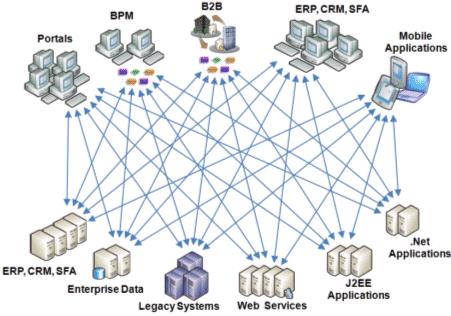
\includegraphics[width=\linewidth]{src/images/03-capitulo-3/tecnologias/esb/point-to-point-integration.png}
  \caption{Diagrama ejemplificando la integración punto a punto}
  \label{fig:point-to-point-integration}
\end{figure}


\subsubsection{El ESB como mediador}

% página 50 SOA in Practice - 5.3.1 Point-to-Point Connections Versus Mediation
% agregar figua con topología de interconexión entre aplicaciones, topología en malla

En una arquitectura en la que se implemente un \gls{acro:esb}, las aplicaciones se comunican a través de este bus central, que actúa como \eng{message broker} entre ellas. Este esquema arquitectónico se llama ``Mediación'' (\eng{Mediation}). De esta manera se reduce el número de conexiones punto a punto que se necesitan para permitir las comunicaciones entre aplicaciones. Al reducir el número de puntos de contacto entre las diferentes aplicaciones, se simplifica el proceso de mantenimiento y actulización de un sistema, decrementando el grado de dependencia directa que pueda existir entre cada instancia.


\subsubsection{El ESB como interceptor}

La otra forma donde un \gls{acro:esb} basado en un protocolo de punto a punto puede proporcionar indirección a las llamadas de servicio, es proporcionando los llamados \eng{interceptors} o \eng{proxies}. Estos elementos, que forman parte del \gls{acro:esb}, se ubican por delante de los servicios existentes y delegan en ellos las peticiones, pero sólo luego de procesarlas ellos y decidir la mejor forma de tratarlas. Un enfoque sencillo es reemplazar el \eng{endpoint} físico que ofrece un servicio, con \eng{hardware} o \eng{software} que sirva como balanceador de carga. Los consumidores siguen utilizando un \eng{endpoint} oficial, donde se delega la verdadera tarea, solo que cuando los mensajes llegan, el interceptor los distribuye a los diferentes proveedores de servicios\cite[p.~52]{josuttis2007}.

\begin{figure}[H]
  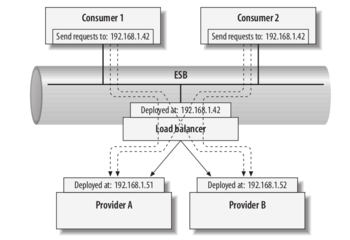
\includegraphics[width=\linewidth]{src/images/03-capitulo-3/tecnologias/esb/esb-interceptors-load-balancer.png}
  \caption{Un ESB como interceptor balancea la carga de los proveedores de servicios}
  \label{fig:esb-interceptors-load-balancer}
\end{figure}
